\chapter{To replace section 5.5 and 5.6}

\section{$\it{CP}$ fit on data}
After the $\it{CP}$ fit procedures from the previous sections 5.1 to 5.5 is reviewed by Belle II collaboration, the permission of measuring $\it{CP}$ parameters using Belle II 2019 and 2020 Spring/Summer data is granted by the review committee. The event number used for the $\it{CP}$ fit is 26, and the fit result is shown as: 

\begin{figure}[H]
\centering
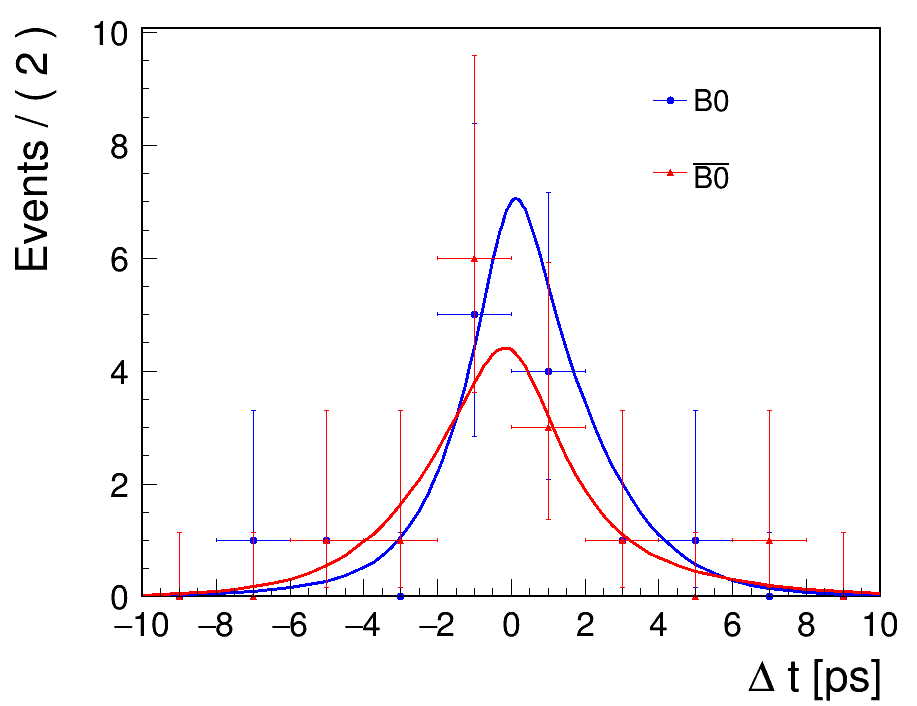
\includegraphics[height=6cm]{cpfit-data}
\caption{The $\it{CP}$ fit using 26 events from data.}
\end{figure}

The results of $\it{CP}$ parameters are: 

\begin{equation}
\begin{split}
sin(2\phi_1) & = 0.71 \pm 0.72(stat) \\
\mathcal{A} & = -0.15 \pm 0.33(stat)\\
\end{split}
\end{equation} 

\section{Systematic Uncertainty}
The systematic uncertainty that affects the fit results may come from many aspects of the measurement setup. 
In this measurement considering the options we used for signal extraction, vertexing and fit strategy, the major systematic uncertainty receives contribution from following points:

\begin{itemize}
	\item resolution functions parameters
	\item signal fraction
	\item flavor tagging 
	\item background $\Delta t$ shapes
	\item fit bias
	\item physics parameters
\end{itemize}
For the above sources of systematic uncertainty, if the parameters are defined with MC study, we float the value by $\pm 2 \sigma$ of their uncertainty, and if the parameters are defined by data, we float the value by $\pm 1 \sigma$, to have a more robust estimation of impact on fit results. The impact of $\it{CP}$ parameters are separately estimated from each sources with positive and negative differentials. With sum of the quadrature of each term, the overall systematic uncertainty is obtained. 

The signal resolution functions' parameters are determined from MC study for signal component. The impact on fit results is summarized as follows: 
\begin{table}[H]
	\begin{minipage}[b]{1.0\linewidth}
		\centering
		\caption{systematic uncertainty from background $\Delta t$ shapes}
		\begin{tabular}{c c c c c}
			\hline
			source & $+\delta \mathcal{S}$ & $+\delta \mathcal{A}$ & $-\delta \mathcal{S}$ &  $-\delta \mathcal{A}$\\
			$f_{cp}^{tail}$ & -0.000096 & -0.000057
& 0.000014
& 0.000056
\\
			$s_0^{main}$& 0.005443
& 0.001299
& -0.005675
& -0.001404
\\
			$s_1^{main}$ & 0.019934
& -0.000903
& -0.020204
& 0.000633
\\
			$s_0^{tail}$ &  -0.003233
& -0.001623
& 0.00327
& 0.001596
\\
			$f_{tag}^{tail}$ & 0.00314
& -0.001257
& -0.003117
& 0.001266
\\
			$s_0^{main}$&  0.002011
& -0.001395
& -0.001956
& 0.001398
\\
			$s_1^{main}$ & 0.005059
& -0.00084
& -0.004969
& 0.000825
\\
			$s_0^{tail}$ &  -0.000135
& -0.000393
& 0.00010 & 0.000435
\\
			$s_1^{tail}$  & 0.000101 & 0.000027 &  -0.000472
& 0.000129
\\
			$f_{\delta}$ & -0.007248
& -0.000552
& 0.007231
& 0.000591
\\
			$f_p$ &  0.003037
& 0.004347
& -0.003069
& -0.004314
\\
			$\tau_n$ & -0.00101 & -0.002841
& 0.000937
& 0.00294
\\
			$\tau_p$ &  0.004497
& 0.002502
& -0.004648
& -0.002478
			\\
			\hline
		\end{tabular}
	\end{minipage}
\end{table}
The background $\Delta t$ shapes' parameters are determined from data sideband $M_{bc}<5.26$ GeV. The impact on fit results is summarized as follows: 
\begin{table}[H]
	\begin{minipage}[b]{1.0\linewidth}
		\centering
		\caption{systematic uncertainty from resolution models}
		\begin{tabular}{c c c c c}
			\hline
			source & $+\delta \mathcal{S}$ & $+\delta \mathcal{A}$ & $-\delta \mathcal{S}$ &  $-\delta \mathcal{A}$\\
		$\mu^{bkg}_{\delta}$ & -0.014294
& -0.016581
& 0.006758
& 0.006537
\\
		$\mu^{bkg}_{l}$&  -0.002798
& -0.012567
& 0.003789
& 0.012783
\\
		$\tau_{bkg}$ & 0.001377
& 0.001689
& -0.004159
& 0.000085\\
		$f_{\delta}^{bkg}$ &  -0.011315
& 0.001365
& 0.011187
& -0.001395
\\
		$f^{bkg}_{tail}$  &-0.002661
& 0.00153
& 0.00248
& -0.001368
\\
		$\sigma^{bkg}_{main}$ & 0.0207015
& 0.022041
& -0.0236175
& -0.01569
\\
		$\sigma^{bkg}_{tail}$ & -0.000275 & -0.000159
& 0.000179
& 0.000141
\\
			\hline
		\end{tabular}
	\end{minipage}
\end{table}
The flavor tagging parameters $\Delta w$ in each rbin is determined from signal MC. The impact in each rbin on fit results is summarized as follows: 
\begin{table}[H]
	\begin{minipage}[b]{1.0\linewidth}
		\centering
		\caption{systematic uncertainty from wrong tagging fraction}
		\begin{tabular}{c c c c c}
			\hline
			source & $+\delta \mathcal{S}$ & $+\delta \mathcal{A}$ & $-\delta \mathcal{S}$ &  $-\delta \mathcal{A}$\\
			$w_1$ & -0.0018919
& 0.001911
& 0.0018549
& -0.002004
\\
			$ w_2$ & -0.0016448
& 0.001104
& 0.0016085
& -0.001155
\\
			$ w_3$ & -0.0004899
& 0.001344
& 0.0004726
& -0.001341
\\
			$ w_4$ & 0.0006556
& 0.000264
& -0.0006542
& -0.000255 \\
			$ w_5$ & -0.0001228
& 0.000204
& 0.0001225 &
-0.000195
\\
			$ w_6$ & 0.0000948 & 0.000054 & 0.0000957 & -0.000045 \\
			$ w_7$ & 0.0001911
& -0.000396
& -0.0001907
& 0.000402
\\
			\hline
		\end{tabular}
	\end{minipage}
\end{table}
The physics parameters $\Delta m_d$ and $\tau_{B^0}$ uncertainties are included using the PDG average value. The impact on fit results is summarized as follows: 
\begin{table}[H]
	\begin{minipage}[b]{1.0\linewidth}
		\centering
		\caption{systematic uncertainty from  physics parameters}
		\begin{tabular}{c c c c c}
			\hline
			source & $+\delta \mathcal{S}$ & $+\delta \mathcal{A}$ & $-\delta \mathcal{S}$ &  $-\delta \mathcal{A}$\\
		$\Delta m_d$  & -0.001767
& -0.000687
& 0.001778
& 0.000696
\\
		$\tau_{B^0}$  & -0.004561
& -0.000546
& 0.004565
& 0.000555
\\
		\hline
		\end{tabular}
	\end{minipage}
\end{table}
The signal fraction is determined using 2D fit results of $M_{bc}$ and $\Delta E$ from data. The impact on fit results is summarized as follows: 
\begin{table}[H]
	\begin{minipage}[b]{1.0\linewidth}
		\centering
		\caption{systematic uncertainty from  signal fraction}
		\begin{tabular}{c c c c c}
			\hline
			source & $+\delta \mathcal{S}$ & $+\delta \mathcal{A}$ & $-\delta \mathcal{S}$ &  $-\delta \mathcal{A}$\\
			mu1\_mbc  & 0.000822 &	-0.003888&	-0.0007965&	0.003849
\\
			sigma1\_mbc & 0.0004755&	0.008442&	-0.000628&	-0.008733
\\
			m0\_argus & -0.000707&	0.00414	&0.001448&	-0.005781
\\
			c\_argus & -0.005544&	0.001449&	0.000922&	-0.000078\\
			f1\_de & 0.0278255 &	0.020589&	-0.0192365	&-0.008409
\\
			f2\_de & 0.020809&	0.017649	&-0.0161285	&-0.007005
\\
			mu1\_de & -0.000443&	-0.000153&	0.0004955&	0.000088\\
			mu2\_de -0.000563&	0.001446&	0.0005905&	-0.001446
\\
			mu3\_de & -0.0031635&	-0.000834&	0.003354&	0.000981
\\
			sigma1\_de& -0.0001715&	-0.000966&	0.000206&	0.000906
\\
			sigma2\_de& -0.0031495&	0.002958&	0.0026345&	-0.002475
\\
			sigma3\_de& -0.001926&	-0.00255&	0.0024695&	0.002985
\\
			a0\_cheb & 0.0009515&	0.000057&	-0.0008925&	-0.000102
\\
			N\_sig\_f & -0.0046395&	0.003987&	0.004922&	-0.003504
\\
			\hline
		\end{tabular}
	\end{minipage}
\end{table}
The fit bias uncertainties is determined by the fit error of 100k signal MC events, which is $\delta {\mathcal{S}}=0.0098$ and $\delta {\mathcal{A}}=0.0057$.


\section{Summary}
The $\it{CP}$ parameters measurement study targeting the extraction of asymmetry parameters $\mathcal{S}$ and $\mathcal{A}$ has been conducted. Based on physical $\Delta t$ distribution, the model for $\it{CP}$ fit have been properly built. Importantly, corresponding resolution functions for $\mathcal{P}_{sig}$ and $\mathcal{P}_{bkg}$ are built by separating smearing effects from \textit{CP} and tag side. All the fits takes advantage of event-by-event conditional fit so the model has a good robustness in different measurement quality cases. As for flavor tagging, an algorithm based on FBDT classification is developed and implemented to give the estimated dilution factor $r$. To take a good use of these information, a Belle II $\it{CP}$ fitter is developed to perform the fit on desired parameters. The linearity test and fit pull test shows a reliable performance of the fitter using toy MC study. The actual fit on lifetime using data is also consistent with the PDG value with a relatively large uncertainty due to very small amount of data. 

After the blind fit and test for the $\it{CP}$ parameters measurement is conduced, with the permission from Belle II collaboration, we unblind the data in signal box and perform the $\it{CP}$ fit to extract $\mathcal{S}$ and $\mathcal{A}$. Also, the major sources of systematic uncertainty is estimated. The primary result of $\it{CP}$ parameters in this low luminosity stage are:

\begin{equation}
\begin{split}
\mathcal{S}=- sin(2\phi_1) & = -0.82 \pm 0.85(stat) \pm 0.07(syst) \\
\mathcal{A} & = -0.21\pm 0.28(stat) \pm 0.06(syst)\\
\end{split}
\end{equation}  

The results are dominated by the statistical uncertainty due to the very limited data sample in early stage of Belle II. Under such large uncertainty, the results is in an agreement with the Standard Model. 
